%%%%%%%%%%%%%%%%%%%%%%%%%%%%%%%%%%%%%%%%%
% Stylish Article - RITA template (SelfArx)
% Election forensics of the 2026 Brazilian presidential election
%%%%%%%%%%%%%%%%%%%%%%%%%%%%%%%%%%%%%%%%%

\documentclass[fleqn,10pt]{SelfArx}
\usepackage[english]{babel}
\usepackage{url}
\usepackage{balance}
\usepackage{hyperref}
\usepackage{mathptmx}
\usepackage{graphicx}
\usepackage{times}
\usepackage{textcomp}
\usepackage{gensymb}
\usepackage{amsmath}
\usepackage{comment}
\usepackage{multirow}
\usepackage[framemethod=tikz]{mdframed}
\usepackage[labelfont=bf]{subcaption}
\usepackage{array}
\usepackage{tikz}
\usetikzlibrary{arrows.meta,positioning}
\newcolumntype{L}[1]{>{\raggedright\arraybackslash}p{#1}}
\newcolumntype{C}[1]{>{\centering\arraybackslash}p{#1}}

\usepackage{tcolorbox}
\definecolor{mycolor}{rgb}{0,0,0}
\makeatletter
\newcommand{\mybox}[1]{%
	\setbox0=\hbox{#1}%
	\setlength{\@tempdima}{\dimexpr\wd0+13pt}%
	\begin{tcolorbox}[colframe=mycolor,boxrule=0.5pt,arc=4pt,
		left=6pt,right=6pt,top=6pt,bottom=6pt,boxsep=0pt,width=\@tempdima]
		#1
	\end{tcolorbox}
}
\makeatother
\usepackage[resetlabels,labeled]{multibib}
\newcites{A}{Appendix}
\usepackage[num]{abntex2cite}
\citebrackets[]

\setlength{\columnsep}{0.55cm}
\setlength{\fboxrule}{0.75pt}
\definecolor{color1}{RGB}{0,0,90}
\definecolor{color2}{RGB}{0,20,20}
\hypersetup{hidelinks,colorlinks,breaklinks=true,urlcolor=color2,citecolor=color1,linkcolor=color1,bookmarksopen=false,
pdftitle={Statistical forensics of the 2026 Brazilian presidential election at the polling-section level},
pdfauthor={C. A. C. Moreira}}

%----------------------------------------------------------------------------------------
%	ARTICLE INFORMATION
%----------------------------------------------------------------------------------------
\JournalInfo{\color{gray}\normalsize\sffamily\bfseries Revista de Informática Teórica e Aplicada - RITA - ISSN 2175-2745\\ Vol.~XX, Num.~XX~(YYYY)~XX-XX}
\Archive{\mybox{RESEARCH ARTICLE}}

\PaperTitle{Statistical Forensics of the 2026 Brazilian Presidential
Election at the Polling-Section Level: a CRISP-DM Application to the
Electoral Court's Open Data}

\ShortTitle{Statistical forensics of the 2026 Brazilian presidential election}

\Titulo{Forense Estatística da Eleição Presidencial Brasileira de 2026
por Seção Eleitoral: uma Aplicação da Metodologia CRISP-DM aos Dados
Abertos do TSE}

\PaperVol{XX}
\PaperNum{X}
\PaperAno{YYYY}

\Authors{C\'esar A. C. Moreira\textsuperscript{1}*}
\affiliation{\textsuperscript{1}\textit{Programa de P\'os-Gradua\c{c}\~ao
em Computa\c{c}\~ao Aplicada (PPCA), Universidade de Bras\'ilia (UnB),
Bras\'ilia, DF, Brasil}}
\affiliation{*\textbf{Autor correspondente}:
cesar.moreira@aluno.unb.br}

\Keywords{Election forensics --- CRISP-DM --- Open government data ---
Electronic voting --- Benford's law --- Electoral integrity}
\newcommand{\keywordname}{Keywords}

\PalavrasChave{Forense eleitoral --- CRISP-DM --- Dados abertos ---
Urna eletr\^onica --- Lei de Benford --- Integridade eleitoral}

\Doi{http://dx.doi.org/10.22456/2175-2745.XXXX}
\DateR{dd/mm/yyyy}
\DateA{dd/mm/yyyy}

%----------------------------------------------------------------------------------------
%	ABSTRACT
%----------------------------------------------------------------------------------------
\Abstract{Brazil publishes the vote count of every polling section,
which allows anyone to test whether the counts follow the statistical
regularities expected from an unmanipulated tally. We applied eight
forensic tests to the 2026 presidential election (first round on
4~October, 499,206 sections; runoff on 25~October, 499,205 sections),
using the Superior Electoral Court (TSE) open data and the six phases of
CRISP-DM. Every test was first validated on synthetic sections with and
without inserted frauds. Votes matched turnout in every section. Last-digit,
second-digit and integer-percentage tests stayed within the expected range
for both finalists; sections at the same polling place were only 1.23--1.26
times more dispersed than random allocation of voters; and the first-round
profile explained 93\% of the within-municipality variance of the runoff
($R^2=0.93$). The turnout--vote fingerprint showed no smear toward the
100\%/100\% corner, and within-municipality turnout was \emph{negatively}
correlated with the winner's share ($r=-0.07$). Crossing the turnout change
between rounds with the unexplained change in vote profile produced a small
monotonic gradient (Spearman $\rho=0.045$; at most 0.22 percentage points),
with opposite signs in 9 of 28 units; among the 158 extreme sections that
gained voters, 88 shifted toward one finalist and 70 toward the other
(binomial $p=0.18$). The remaining outliers (about 0.01\% of sections)
concentrate in indigenous villages, prisons, sections abroad and a few urban
sections, and mostly repeat across rounds. We list the sections for manual
check against the printed tally and propose twelve further tests, including
a full recount of the digital vote record.}

\Resumo{O Brasil publica a contagem de votos de cada se\c{c}\~ao eleitoral,
o que permite testar se as contagens seguem as regularidades estat\'isticas
esperadas em uma apura\c{c}\~ao sem manipula\c{c}\~ao. Aplicamos oito testes
forenses \`a elei\c{c}\~ao presidencial de 2026 (1\textordmasculine{} turno
em 4 de outubro, 499.206 se\c{c}\~oes; 2\textordmasculine{} turno em 25 de
outubro, 499.205 se\c{c}\~oes), com os dados abertos do Tribunal Superior
Eleitoral (TSE) e as seis fases do CRISP-DM. Cada teste foi validado antes
com se\c{c}\~oes sint\'eticas com e sem fraudes inseridas. Os votos
coincidiram com o comparecimento em todas as se\c{c}\~oes. Os testes de
\'ultimo d\'igito, de segundo d\'igito e de percentuais inteiros ficaram
dentro do esperado para os dois finalistas; se\c{c}\~oes do mesmo local de
vota\c{c}\~ao foram apenas 1,23 a 1,26 vez mais dispersas que uma
aloca\c{c}\~ao aleat\'oria de eleitores; e o perfil do 1\textordmasculine{}
turno explicou 93\% da vari\^ancia do 2\textordmasculine{} turno dentro do
munic\'ipio. A ``impress\~ao digital'' comparecimento--voto n\~ao mostrou
deslocamento para o canto 100\%/100\%, e o comparecimento dentro do
munic\'ipio foi \emph{negativamente} correlacionado com a vota\c{c}\~ao do
vencedor ($r=-0,07$). O cruzamento entre a varia\c{c}\~ao de comparecimento
e a mudan\c{c}a n\~ao explicada de perfil entre turnos mostrou um gradiente
pequeno (Spearman $\rho=0,045$; no m\'aximo 0,22 ponto percentual), com sinal
oposto em 9 de 28 unidades; entre as 158 se\c{c}\~oes extremas que ganharam
eleitores, 88 se deslocaram para um finalista e 70 para o outro (binomial
$p=0,18$). Os casos extremos restantes (cerca de 0,01\% das se\c{c}\~oes)
concentram-se em aldeias ind\'igenas, pres\'idios, se\c{c}\~oes no exterior
e poucas se\c{c}\~oes urbanas, e em geral se repetem nos dois turnos.
Listamos as se\c{c}\~oes para confer\^encia no Boletim de Urna e propomos
doze novos testes, entre eles a recontagem integral do Registro Digital do
Voto.}

%----------------------------------------------------------------------------------------
\begin{document}

\flushbottom
\maketitle
\thispagestyle{empty}

%======================================================================
\section{Introduction}
\label{sec:intro}

Brazil publishes the result of every polling section (\emph{se\c{c}\~ao
eleitoral}), so anyone can reproduce the national tally and test whether
the counts behave as an unmanipulated count should. For the 2026 general
election the Superior Electoral Court (TSE) released, besides the tally
sheet (\emph{Boletim de Urna}, BU), the digital vote record (\emph{Registro
Digital do Voto}, RDV) and the log of each voting machine, as well as
consolidated files in its Open Data Portal \cite{tse2026}.

Election forensics is the branch of statistics that searches such data for
the marks that manipulation tends to leave: invented numbers, rounded
percentages, coordinated inflation of turnout in some sections, or swings
that only a few sections show \cite{hicken2017,klimek2012}. In Brazil,
Figueiredo Filho, Silva and Carvalho \cite{figueiredo2022} applied five such
tests to the 2018 presidential election, and an election-fingerprint
analysis of the 2022 runoff found no statistical sign of ballot stuffing or
voter rigging \cite{csh2022}.

This article applies and extends that line of work to the 2026 presidential
election. Three research questions guide the study:
\textbf{RQ1} --- do section-level counts follow the regularities expected
from an unmanipulated tally?;
\textbf{RQ2} --- where there are deviations, are they systematic or
isolated, and do they have a plausible demographic explanation?; and
\textbf{RQ3} --- are the changes in turnout and in vote profile between the
first round and the runoff consistent with each other?

\paragraph{Contributions} (i) a reproducible CRISP-DM pipeline, in R, that
validates every test on synthetic data with known inserted frauds before
using it on real data; (ii) the use of \emph{local} references --- the other
sections of the same polling place or municipality --- instead of national
medians, which removes the regional false alarms we found in a first
version; (iii) a new cross-round test (T8) that relates the change in
turnout of each section to the part of its vote change that the
first-round composition does not explain, with a symmetry test between the
two finalists; and (iv) a list of flagged sections, classified by the name
of the polling place, ready for manual verification.

The study is statistical and exploratory. An unusual pattern indicates
where to look; it does not prove irregularity. Likewise, the absence of a
pattern does not prove that no irregularity occurred.

%======================================================================
\section{Theoretical Background}
\label{sec:background}

Each forensic test starts from a regularity that honest counts tend to
follow and that counts invented or altered by people tend to violate.
Table~\ref{tab:tests} summarizes the tests used here and the main known
limitation of each.

\begin{table*}[ht]
\caption{Forensic tests used in this study}
\label{tab:tests}
\centering\small
\begin{tabular}{@{}L{2.6cm} L{5.0cm} L{4.6cm} L{3.6cm}@{}}
\toprule
\textbf{Test} & \textbf{Expected regularity} & \textbf{Known limitation} & \textbf{Reference} \\
\midrule
T1 Zeros and 100\% & Few unanimous sections where the candidate has intermediate support & Isolated communities are genuinely unanimous & \cite{hicken2017} \\
T2 Last digit & Digits 0--9 with 10\% each in counts with two or more digits & Biased when there are few votes per section & \cite{beber2012,mack2019} \\
T3 Second digit (2BL) & Benford distribution of the second digit, mean 4.187 & Rejects under normal strategic voting & \cite{mebane2008,deckert2011,pericchi2011} \\
T4 Integer percentages & Frequency of integer percentages equal to binomial simulations & Simple fractions create spikes in small sections & \cite{kobak2016,rozenas2017} \\
T5 Local homogeneity & Sections of the same polling place are similar & Voters are not randomly assigned to sections & This study (quasi-binomial) \\
T6 Cross-round consistency & Runoff share predicted by the section's own first round; stable turnout & Transit and transferred voters change the electorate & This study; \cite{klimek2023} \\
T7 Fingerprint & No smear of turnout and leader share toward 100\%/100\% & Needs eligible voters per section & \cite{klimek2012,klimek2018} \\
T8 Turnout $\times$ profile & No link between extra turnout and unexplained shift & Ecological regression assumptions & This study; \cite{goodman1953} \\
\bottomrule
\end{tabular}
\end{table*}

The first-digit Benford test was not used. Sections have bounded size,
roughly between 100 and 400 voters, and in that range the law does not hold
even for clean data \cite{deckert2011}.

Two statistical cautions run through the whole study. First, with hundreds
of thousands of sections any tiny deviation yields $p<0.001$, so effect
size matters more than the $p$-value. Second, when testing section by
section, the false discovery rate must be controlled \cite{benjamini1995}
and the over-dispersion between sections must be corrected; outliers are
measured with robust $z$-scores based on the median and the median absolute
deviation \cite{leys2013}.

%======================================================================
\section{Related Work}
\label{sec:related}

The literature on election forensics can be organized into four strands:
digit tests, distributional tests on vote shares and turnout, cross-round or
cross-election comparisons, and supervised learning on synthetic frauds.
Table~\ref{tab:related} compares the studies closest to ours.

\paragraph{Digit tests} Mebane \cite{mebane2008} proposed the second-digit
Benford test (2BL) for precinct counts in United States presidential
elections. Pericchi and Torres \cite{pericchi2011} applied first- and
second-digit tests, plus a version restricted to bounded units, to
elections in the United States, Puerto Rico and Venezuela; the second-digit
law was clearly rejected only in the 2004 Venezuelan recall referendum and
only for electronic voting units. Beber and Scacco \cite{beber2012} moved
the focus to last digits and digit pairs, exploiting the biases people show
when inventing numbers. Deckert, Myagkov and Ordeshook \cite{deckert2011}
showed that Benford-type tests can fail in both directions, and an
experiment by Mack and Stoetzer \cite{mack2019}, in which participants
were paid to alter tally sheets without being detected, found that
last-digit tests do not reliably identify manipulated counts. These results
are why we treat T2 and T3 as weak evidence and calibrate them by
simulation.

\paragraph{Vote-share and turnout distributions} Klimek et al.\
\cite{klimek2012} introduced the turnout--vote \emph{fingerprint} and a
model of ballot stuffing and voter rigging; the same group later found
fingerprints of ballot stuffing in about 11\% of Turkish polling stations in
the 2017 referendum \cite{klimek2018}. Kobak, Shpilkin and Pshenichnikov
\cite{kobak2016} showed that falsified Russian results contain an excess of
integer percentages, and Rozenas \cite{rozenas2017} proposed a resampled
kernel-density method that separates such spikes from those created by
small units. Leemann and Bochsler \cite{leemann2014} argued for testing
several empirical implications of different forms of fraud together and
discussed how to handle the resulting multiple comparisons, a point we
follow with the Benjamini--Hochberg procedure.

\paragraph{Cross-round comparisons} Closest to our T6 and T8, Klimek, Ayka\c{c}
and Thurner \cite{klimek2023} compared the two rounds of the 2023 Turkish
presidential election at the ballot-box level and found that districts with
few ballot boxes were more likely to show large vote swings toward the
incumbent between rounds. Their test is about the size of the swing in
remote units; ours relates the swing that the first round does not explain
to the change in turnout and tests whether extreme cases favour one side.

\paragraph{Machine learning on synthetic frauds} Cant\'u and Saiegh
\cite{cantu2011} trained a classifier on synthetic clean and manipulated
elections and applied it to Argentina in the 1930s; Zhang, Alvarez and Levin
\cite{zhang2019} used random forests trained on synthetic data to flag
polling places in Argentina's 2015 election. Cant\'u \cite{cantu2019} used
convolutional neural networks on images of about 50,000 tally sheets from
Mexico's 1988 election and found blatant alterations in about a third of
them, showing the value of checking the physical record and not only the
published numbers. Our validation step borrows the idea of synthetic frauds,
but uses it to calibrate and debug classical tests rather than to train a
classifier.

\paragraph{Brazil} Figueiredo Filho, Silva and Carvalho
\cite{figueiredo2022} applied five tests (2BL, last-digit mean, frequency of
last digits 0 and 5, correlation between vote share and turnout, and
resampled kernel density) to the 2018 presidential election at the section
and municipality levels and found no evidence of fraud. For the 2022
runoff, Klimek and Thurner \cite{csh2022} analysed 471,983 units and found
no fingerprints of ballot stuffing or voter rigging, and Nogueira
\cite{nogueira2024} discussed statistical methods and electoral integrity in
the 2022 Brazilian elections. Other Brazilian applications of Benford's law
target different objects: campaign donations \cite{gamermann2018} and
Senate elections from 1994 to 2018 with a change of numerical base
\cite{gueron2022}.

\paragraph{Gap} Previous Brazilian studies analysed one round at a time,
used national references, and did not report how each test behaves on data
with known frauds. This study analyses both rounds, links them section by
section, uses local references, validates every test on synthetic frauds
before using real data, and identifies the flagged sections by the name of
the polling place.

\begin{table*}[ht]
\caption{Related studies at the polling-unit level}
\label{tab:related}
\centering\small
\begin{tabular}{@{}L{3.3cm} L{3.0cm} L{4.6cm} L{5.0cm}@{}}
\toprule
\textbf{Study} & \textbf{Election(s)} & \textbf{Methods} & \textbf{Main finding} \\
\midrule
Pericchi and Torres \cite{pericchi2011} & USA, Puerto Rico, Venezuela & First- and second-digit Benford, restricted version & 2BL rejected only for Venezuela 2004 electronic units \\
Cant\'u and Saiegh \cite{cantu2011} & Argentina 1931--1941 & Naive Bayes trained on synthetic data & Historically irregular elections classified as fraudulent \\
Klimek et al.\ \cite{klimek2012} & Several countries & Turnout--vote fingerprint, fraud model & Fingerprints of ballot stuffing in some countries \\
Beber and Scacco \cite{beber2012} & Several, incl.\ Nigeria & Last digits and digit pairs & Human-invented counts leave digit traces \\
Leemann and Bochsler \cite{leemann2014} & Swiss referendum 2011 & Several tests, multiple-comparison control & Irregularities in municipalities that destroyed ballots \\
Kobak et al.\ \cite{kobak2016} & Russia & Integer percentages & Excess of round percentages \\
Klimek et al.\ \cite{klimek2018} & Turkey 2017--2018 & Fingerprint, fraud model & Ballot stuffing in about 11\% of stations (2017) \\
Zhang et al.\ \cite{zhang2019} & Argentina 2015 & Random forest on synthetic data & Polling places at risk flagged \\
Cant\'u \cite{cantu2019} & Mexico 1988 & CNN on tally-sheet images & Alterations in about a third of tallies \\
Figueiredo Filho et al.\ \cite{figueiredo2022} & Brazil 2018 & Five tests (digits, turnout, kernel) & No evidence of fraud \\
Klimek and Thurner \cite{csh2022} & Brazil 2022, runoff & Fingerprint, ballot stuffing and rigging & No signs of fraud \\
Klimek et al.\ \cite{klimek2023} & Turkey 2023, two rounds & Fingerprint, cross-round swings & Extreme swings in remote areas \\
\textbf{This study} & \textbf{Brazil 2026, two rounds} & \textbf{T1--T8 with synthetic validation, local references, cross-round turnout $\times$ profile} & \textbf{See Sections~\ref{sec:results}--\ref{sec:cross}} \\
\bottomrule
\end{tabular}
\end{table*}

%======================================================================
\section{Methodology}
\label{sec:method}

The study followed the six phases of CRISP-DM \cite{chapman2000,wirth2000},
with the evaluation phase carried out \emph{before} the use of real data
(Figure~\ref{fig:crisp}). All processing was done in R with the
\texttt{data.table} package.

\begin{figure}[ht]
\centering
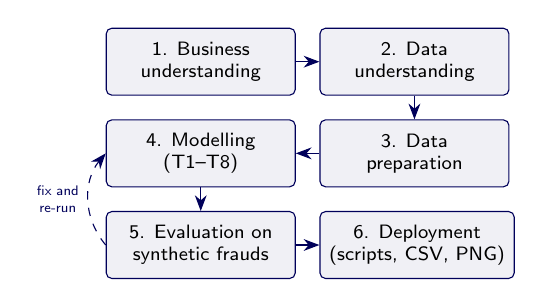
\begin{tikzpicture}[node distance=3mm and 3mm,
  box/.style={draw=color1,rounded corners=2pt,fill=color1!6,align=center,
  font=\sffamily\scriptsize,minimum width=2.4cm,minimum height=0.85cm},
  arr/.style={-{Stealth[length=2mm]},color1}]
\node[box] (b) {1. Business\\understanding};
\node[box,right=of b] (d) {2. Data\\understanding};
\node[box,below=of d] (p) {3. Data\\preparation};
\node[box,below=of b] (m) {4. Modelling\\(T1--T8)};
\node[box,below=of m] (e) {5. Evaluation on\\synthetic frauds};
\node[box,right=of e] (i) {6. Deployment\\(scripts, CSV, PNG)};
\draw[arr] (b)--(d); \draw[arr] (d)--(p); \draw[arr] (p)--(m);
\draw[arr] (m)--(e); \draw[arr] (e)--(i);
\draw[arr,dashed] (e.west) to[bend left=40] node[left,font=\sffamily\tiny,align=center]{fix and\\re-run} (m.west);
\end{tikzpicture}
\caption{CRISP-DM as applied. Evaluation on synthetic data with known
frauds came before the analysis of real data and fed corrections back into
modelling.}
\label{fig:crisp}
\end{figure}

\paragraph{Business understanding} The question is whether section-level
counts have regularities compatible with an unmanipulated tally. The success
criterion is that each test separates clean data from data with inserted
fraud, without false alarms.

\paragraph{Data understanding} The sources are the files ``President ---
vote by polling section'' (\texttt{votacao\_secao\_\allowbreak 2026\_BR}) and ``Count
details by polling section'' (\texttt{detalhe\_votacao\_\allowbreak secao\_2026}),
generated by the TSE on 26~October 2026 \cite{tse2026}. The first has one
row per section, round and candidate, with state (UF), municipality, zone,
section, polling place and votes; blank votes have code 95 and null votes
code 96. The second has eligible voters and turnout per section. State files
contain only state-level offices.

\paragraph{Data preparation} Rows were filtered for the office of President
and converted from Latin-1 to UTF-8. The TSE does not publish rows with zero
votes, so each section was completed with zeros for all candidates of the
round. The section key is UF + municipality + zone + section; valid votes
exclude codes 95, 96 and 97. A load check compared both files: the sum of
votes equals the reported turnout in \emph{every} section of both rounds
(125,275,835 votes in the first round and 128,236,074 in the runoff, for
158,745,502 eligible voters; turnout of 78.9\% and 80.8\%). The detail file
lists 42 extra sections abroad in the first round and 43 in the runoff, all
with eligible voters but zero turnout.

\paragraph{Modelling} Eight tests, T1 to T8, described in
Sections~\ref{sec:results} and \ref{sec:cross}. References are local: the
other sections of the same polling place or municipality, not the national
median. Section-level tests use the Benjamini--Hochberg correction
($q<0.001$) and robust $z$-scores \cite{leys2013}.

\paragraph{Evaluation} We generated 3,559 synthetic sections in the TSE
layout, in two versions. One is clean. The other has three inserted frauds:
8 sections with 100\% for one candidate, 300 sections with a forced integer
percentage and 5 sections with inflated turnout. This step revealed three
faults that were fixed before the real analysis: the theoretical digit
references raised false alarms; the homogeneity test without dispersion
adjustment flagged 75 clean sections; and turnout compared with the national
median confused regional variation with anomaly. Table~\ref{tab:valid}
shows the corrected tests.

\begin{table}[ht]
\caption{Validation on synthetic data (3,559 sections)}
\label{tab:valid}
\centering\small
\begin{tabular}{@{}L{2.6cm} L{1.8cm} L{2.9cm}@{}}
\toprule
\textbf{Test} & \textbf{Clean data} & \textbf{Inserted frauds} \\
\midrule
T1 Zeros and 100\% & no alert & 8 of 8 sections detected \\
T4 Integer \% & ratio 0.95 ($p=0.72$) & ratio 2.86 ($p<0.01$) \\
T5 Local homogeneity & 0 sections & 8 of 8 detected \\
T6 Cross-round & 0 sections & 7 of 8 detected \\
T6 Turnout & 0 sections & 4 flagged, 3 inserted \\
T8 Turnout $\times$ profile & 1 section (lost votes) & 4 of 5 inflated, all ``more votes, toward beneficiary'' \\
\bottomrule
\end{tabular}
\end{table}

\paragraph{Deployment} Three reproducible scripts: download with integrity
check, section-level distribution and the test battery, plus the T8 script.
Results are written as CSV and PNG files, ready for checking against the
tally sheets.

%======================================================================
\section{Results}
\label{sec:results}

Both finalists passed every aggregate regularity test. Deviations appear in
few sections and, in general, repeat the same pattern in both rounds. We
analysed 499,206 sections in the first round and 499,205 in the runoff.

\subsection{Sections with 0\% and 100\% (T1)}

There are more unanimous sections than the binomial model predicts, but the
excess is small in absolute terms (Table~\ref{tab:t1}).

\begin{table}[ht]
\caption{Unanimous sections (T1)}
\label{tab:t1}
\centering\small
\begin{tabular}{@{}c L{2.5cm} r r r@{}}
\toprule
\textbf{Round} & \textbf{Event} & \textbf{Obs.} & \textbf{Exp.} & \textbf{$p$ (Poisson)} \\
\midrule
2nd & 100\% Lula & 106 & 49.7 & $2.7\times10^{-12}$ \\
2nd & 100\% F.\ Bolsonaro & 4 & 2.3 & 0.20 \\
1st & 100\% Lula & 38 & 18.5 & $4.5\times10^{-5}$ \\
1st & 0 votes F.\ Bolsonaro & 81 & 37.4 & $4.6\times10^{-10}$ \\
\bottomrule
\end{tabular}
\end{table}

Three facts point to communities with homogeneous vote rather than to
manipulation. The sections lie mostly in the states of MG (26 sections),
AM (23), MA (22), PA (21) and RS (11) and typically have between 10 and 150
valid votes (median 81). The same sections are
unanimous in both rounds (for instance AM 2690/280, MA 8958/170 and 179, and
PA 4111/516 and 519), and some sections are unanimous for the other
finalist in both rounds (RS 85839/81, PA 4200/44). The expected value
underestimates unanimity because it assumes voters similar to those of
neighbouring sections, which does not hold for villages or isolated
communities.

\subsection{Digit tests (T2 and T3)}

The last digit is uniform for both finalists in both rounds
(Figure~\ref{fig:t2}). The theoretical Benford reference for the second
digit always rejects ($p\approx0$), but the simulated reference shows
deviations of at most 0.12 percentage points (Table~\ref{tab:digits}).

\begin{table}[ht]
\caption{Digit tests with simulated references}
\label{tab:digits}
\centering\small
\begin{tabular}{@{}c l c c c@{}}
\toprule
\textbf{Rd.} & \textbf{Candidate} & \textbf{Last, $p$} & \textbf{2nd, $p$} & \textbf{2nd, max.\ dev.\ (p.p.)} \\
\midrule
1st & Lula & 0.48 & 0.61 & 0.06 \\
1st & F.\ Bolsonaro & 0.67 & 0.015 & 0.09 \\
2nd & Lula & 0.76 & 0.11 & 0.10 \\
2nd & F.\ Bolsonaro & 0.23 & 0.0027 & 0.12 \\
\bottomrule
\end{tabular}
\end{table}

With eight simultaneous tests the Bonferroni threshold is 0.006. Only the
second digit of Fl\'avio Bolsonaro in the runoff falls below it, with a
practically irrelevant effect. Mebane \cite{mebane2008} already notes that
2BL reacts to ordinary strategic behaviour of voters.

\begin{figure}[ht]
\centering
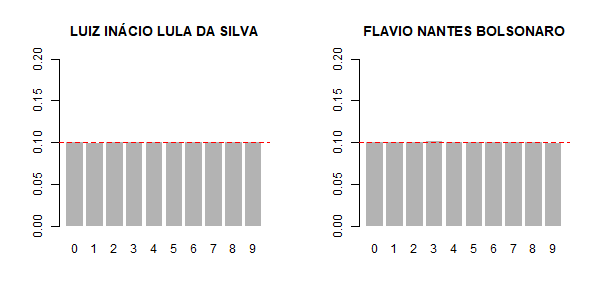
\includegraphics[width=\linewidth]{Figures/T2_ultimo_digito_turno2.png}
\caption{Last digit of the runoff counts for Lula (left) and Fl\'avio
Bolsonaro (right); the dashed line is the 10\% expected under
uniformity.}
\label{fig:t2}
\end{figure}

\subsection{Integer percentages (T4)}

There is no excess of integer percentages in the runoff: observed/expected
ratio 0.995 for both finalists ($p=0.72$ and $0.69$). In the first round
the ratios were 1.014 for Lula ($p=0.059$) and 1.009 for Fl\'avio Bolsonaro
($p=0.18$). Among candidates with enough votes, only Augusto Cury reached
the smallest $p$ possible with 100 simulations (0.0099); his excess is about
250 sections, far below the Russian anomalies described by Kobak et al.\
\cite{kobak2016}. The small peaks near 25\%, 33\% and 50\%
(Figure~\ref{fig:t4}) come from simple fractions in small sections and are
already included in the simulation.

\begin{figure}[ht]
\centering
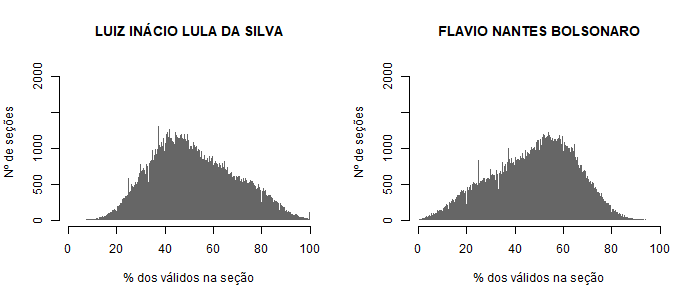
\includegraphics[width=\linewidth]{Figures/T4_histograma_pct_turno2.png}
\caption{Distribution of the share of valid votes per section in the
runoff (x axis: \% of valid votes; y axis: number of sections).}
\label{fig:t4}
\end{figure}

\subsection{Homogeneity within the polling place (T5)}

Sections of the same building are almost as similar as they would be with
randomly assigned voters: the dispersion ratio was 1.23--1.24 in the first
round and 1.26 in the runoff for the finalists. After the quasi-binomial
adjustment and the BH correction, between 67 and 85 sections per candidate
and round differ by at least 20 percentage points, about 0.014\% of the
total. Almost all differ in the same direction and by a similar amount in
both rounds (e.g.\ SP 62499/402, MG 41238/336, MA 9610/468), a pattern
typical of a different electorate in the section, such as a special section
or transferred voters.

\subsection{Consistency between rounds (T6)}

The first round of each section explains 93\% of the variation of the
runoff within the municipality ($R^2=0.9318$), and the scatter is a narrow
band without clusters off the curve (Figure~\ref{fig:t6}).

\begin{figure}[ht]
\centering
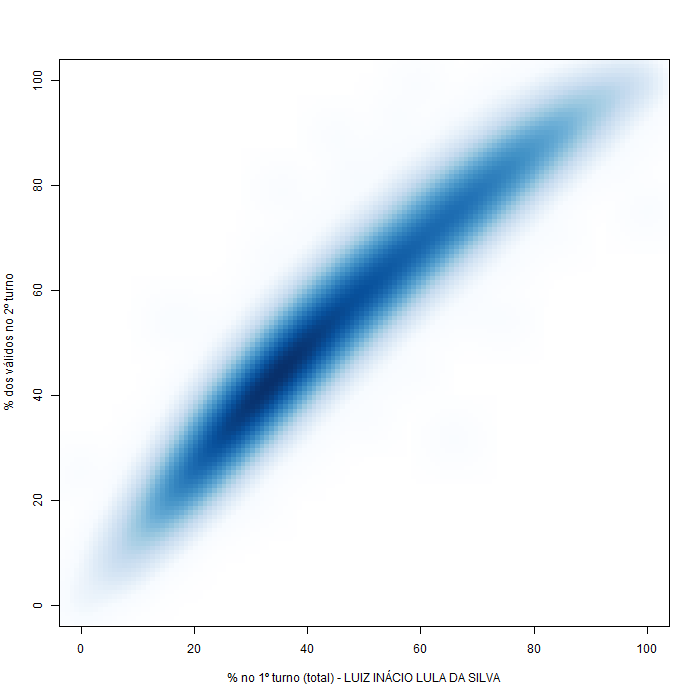
\includegraphics[width=0.85\linewidth]{Figures/T6_1o_x_2o_turno.png}
\caption{Lula's share in the first round (x axis, \% of total) versus his
share of valid votes in the runoff (y axis), per section; density plot.}
\label{fig:t6}
\end{figure}

Fourteen sections deviate from the prediction with robust $|z|\geq6$
(Table~\ref{tab:t6}). Six of them are in indigenous villages or
indigenous lands, according to the polling-place name, and one is abroad
(Porto, Portugal). Four are in the same polling place in S\~ao Paulo
(municipality 71072, zone 2), where Fl\'avio Bolsonaro did better than
predicted and the sections received 16--25\% more votes in the runoff;
they may be sections for voters in transit, since a voter can request
transit voting in only one round. This hypothesis was not verified.

\begin{table}[ht]
\caption{Sections flagged by T6 ($|z|\geq6$)}
\label{tab:t6}
\centering\scriptsize
\begin{tabular}{@{}l r r r L{3.1cm}@{}}
\toprule
\textbf{UF/mun./zone/sec.} & \textbf{Valid} & \textbf{Lula \%} & \textbf{$z$} & \textbf{Polling place (type)} \\
\midrule
AC 1554/3/160 & 152 & 31.6 & $-14.7$ & Health post, Bua\c{c}\'u village (indig.) \\
AM 2097/18/37 & 155 & 54.2 & 13.1 & Municipal school \\
AC 1031/3/95 & 221 & 78.7 & 12.6 & Health unit, Maronawa village (indig.) \\
AM 2399/45/63 & 169 & 98.8 & 11.4 & School, Piau village (indig.) \\
AC 1139/7/67 & 66 & 78.8 & 10.6 & Nova Floresta village (indig.) \\
PI 11878/28/99 & 268 & 54.5 & $-9.7$ & Rural school \\
SP 71072/2/519 & 293 & 55.3 & $-7.1$ & School (same site) \\
SP 71072/2/539 & 312 & 64.1 & $-7.1$ & School (same site) \\
MA 8974/70/403 & 127 & 88.2 & 6.9 & Zemuehan Tentenhar school (indig.) \\
BA 34134/170/262 & 60 & 66.7 & 6.8 & School \\
SP 71072/2/491 & 308 & 51.3 & $-6.6$ & School (same site) \\
SP 71072/2/532 & 313 & 56.2 & $-6.5$ & School (same site) \\
PA 4723/80/254 & 162 & 97.5 & 6.3 & Trincheira Bacaj\'a school (indig.) \\
ZZ 30341/1/3576 & 251 & 64.9 & 6.0 & Porto, Portugal (abroad) \\
\bottomrule
\end{tabular}
\end{table}

\paragraph{Turnout change} The first version of the turnout test compared
each section with the national median and flagged 2,088 sections, which
were in fact whole states (AC, AP, RR, MA and PA) where turnout fell in the
runoff. The corrected version compares each section with its own
municipality. It flagged 730 sections (0.15\%) with robust $|z|\geq6$ on
the log-ratio of votes between rounds: 574 with \emph{fewer} votes in the
runoff and 156 with more. A keyword classification of the polling-place
names (approximate; script \texttt{classificar\_locais\_t6.R}) found 54
prisons or juvenile detention units, 53 of them losing voters, consistent
with releases and transfers of inmates between rounds; 53 indigenous
villages, 40 of them gaining voters; 18 hospitals or care homes; and 18
sections abroad, 17 of them gaining voters. The flagged sections concentrate in PA
(128), AC (85), AM (68), MA (67) and AP (64). The largest increases occurred
in indigenous schools in PA and MS (e.g.\ PA 4111/18/519, from 21 to 35
votes; PA 5835/106/330, from 128 to 212) and in the embassy in Canberra
(from 72 to 111).

\subsection{Turnout--vote fingerprint (T7)}

The two-dimensional histogram of turnout and leader share
(Figure~\ref{fig:t7}) shows a single compact cloud centred around 80\%
turnout, elongated along the vote axis, without the smear toward the
100\%/100\% corner that characterizes ballot stuffing
\cite{klimek2012,klimek2018}. Within municipalities, turnout was
\emph{negatively} correlated with Lula's share ($r=-0.095$ in the first
round and $r=-0.069$ in the runoff) and positively with Fl\'avio
Bolsonaro's ($r=0.086$ and $0.069$). Ballot stuffing in favour of the winner
would produce the opposite sign. Sections with turnout $\geq95\%$ and
share $\geq95\%$ for the same candidate are rare: 26 (first round) and 64
(runoff) for Lula and 1 and 2 for Fl\'avio Bolsonaro, i.e.\ at most 0.013\%
of sections; they are likely the same small homogeneous sections found by
T1, which remains to be confirmed. Integer turnout percentages were not in
excess: 7,635 observed versus 7,581.5 expected in the first round
($p=0.27$) and 7,088 versus 7,155.4 in the runoff ($p=0.85$).

\begin{figure}[ht]
\centering
\begin{subfigure}{0.49\linewidth}
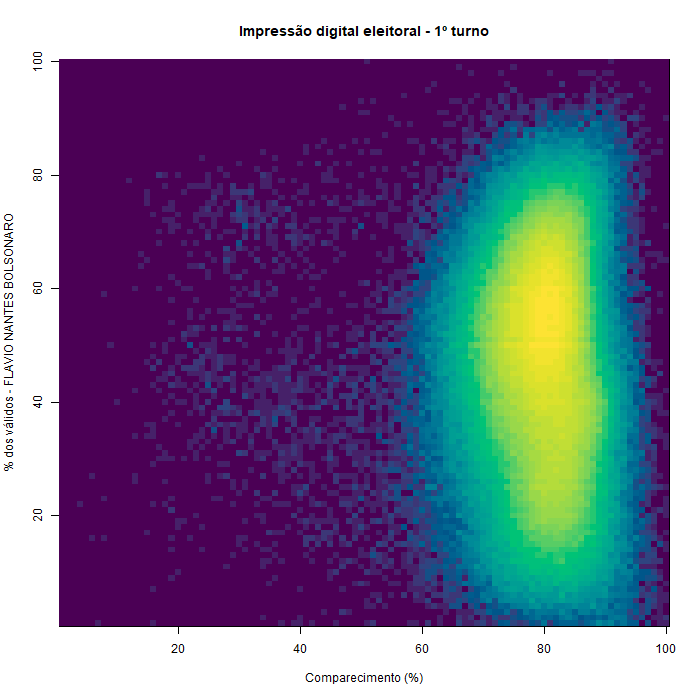
\includegraphics[width=\linewidth]{Figures/T7_impressao_digital_turno1.png}
\caption{First round, F.\ Bolsonaro}
\end{subfigure}
\begin{subfigure}{0.49\linewidth}
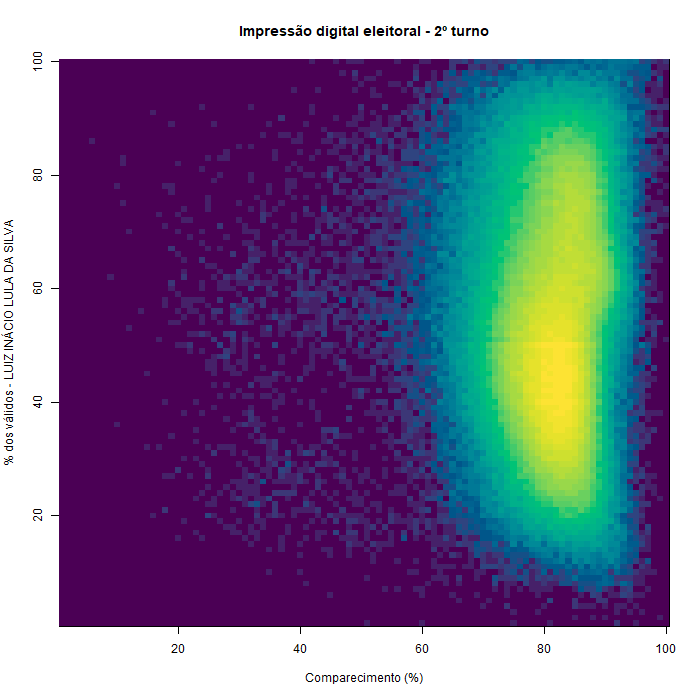
\includegraphics[width=\linewidth]{Figures/T7_impressao_digital_turno2.png}
\caption{Runoff, Lula}
\end{subfigure}
\caption{Election fingerprints: turnout (x axis, \%) versus the share of
valid votes of the round leader (y axis, \%); brighter means more
sections.}
\label{fig:t7}
\end{figure}

%======================================================================
\section{Cross-analysis: Turnout $\times$ Change of Vote Profile (T8)}
\label{sec:cross}

T8 tests whether sections whose turnout changed more than their neighbours'
also changed their vote disproportionately. Inflating a section with votes
for a single candidate leaves exactly that mark: more votes and a profile
shifted toward the same side \cite{klimek2012}.

For each section present in both rounds with at least 30 votes in each, two
measures are computed, both centred on the municipality median, using only
municipalities with three or more sections:
\begin{equation}
\Delta C_s = \ln\!\left(\frac{V_{2,s}}{V_{1,s}}\right), \qquad
\Delta P_s = 100\,\bigl(p_{2,s}-\hat{p}_{2,s}\bigr),
\end{equation}
where $V$ is the section total in each round (including blank and null
votes), $p_2$ is the share of finalist A (Lula) among the two finalists in
the runoff, and $\hat{p}_2$ is the prediction of that share from the
first-round composition of the same section (votes for A, for B, for other
candidates, and blank or null), obtained from a transfer regression
estimated by state \cite{goodman1953}. $\Delta P$ thus measures the part of
the profile change that the first round does not explain.

\paragraph{Deciles} Figure~\ref{fig:t8dec} shows the mean of $\Delta P$ per
decile of $\Delta C$. The curve is not flat: it rises from $-0.09$ to
$+0.22$ percentage points, so sections whose turnout grew most relative to
their municipality shifted slightly toward Lula, and those whose turnout
fell most shifted slightly toward Fl\'avio Bolsonaro. The effect is
statistically clear (non-overlapping 95\% intervals at the extremes) but
small: two tenths of a percentage point in the top decile, where turnout
grew 5.1\% above the municipal median.

\begin{figure}[ht]
\centering
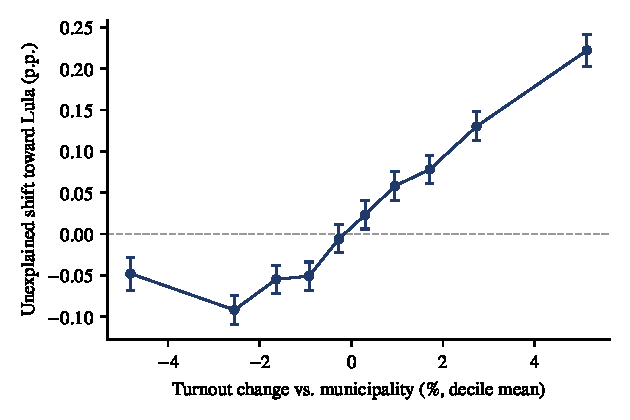
\includegraphics[width=\linewidth]{Figures/fig_t8_deciles.pdf}
\caption{Mean unexplained shift toward Lula ($\Delta P$, with 95\% CI) per
decile of turnout change relative to the municipality ($\Delta C$);
498,952 sections.}
\label{fig:t8dec}
\end{figure}

\paragraph{Correlation by state} The national Spearman correlation between
$\Delta C$ and $\Delta P$ is $\rho=0.045$ (0.031 without centring). It
varies in sign across units (Figure~\ref{fig:t8uf}): it is positive in 19
and negative in 9 of the 28 units, ranging from $-0.10$ (AP and AC) to
$+0.16$ (sections abroad), with the largest positive values in the South
and Centre-West (SC, MS, PR, DF, MT). A coordinated manipulation in favour
of one candidate would push all states in the same direction; the mixed
signs are more consistent with regional differences in which groups of
voters were mobilized or demobilized between rounds.

\begin{figure}[ht]
\centering
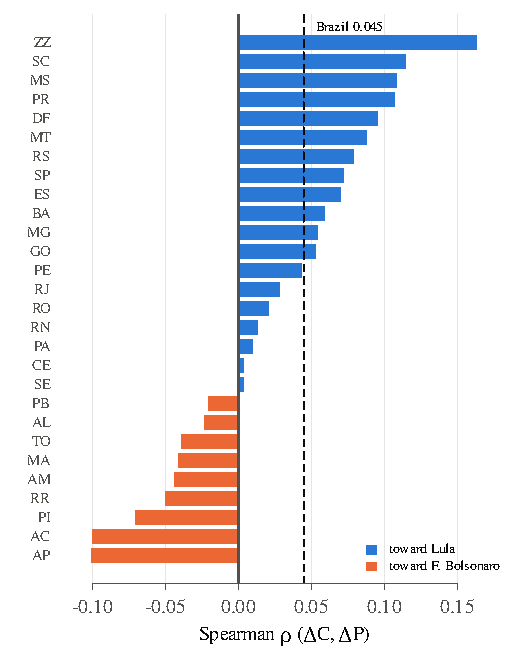
\includegraphics[width=\linewidth]{Figures/fig_t8_uf.pdf}
\caption{Spearman correlation between $\Delta C$ and $\Delta P$ by state
(ZZ = abroad). Dashed line: national value.}
\label{fig:t8uf}
\end{figure}

\paragraph{Vote transfer} The national ecological regression estimates that
first-round voters of each finalist stayed with him (coefficients 1.03 and
1.01), voters of other candidates split evenly (0.44 to each), blank and
null voters went mostly to Lula (0.63), and the extra runoff voters split
0.55 to Lula and 0.41 to Fl\'avio Bolsonaro. In 9 units at least one
coefficient fell outside $[0,1]$ by more than 0.05, mostly Lula retention
rates of 1.05--1.08 in SP, the South and the Centre-West. This indicates
that the constant-transfer assumption of Goodman's regression does not fit
there, a known limitation of ecological inference, not an impossible count.

\paragraph{Flagged sections and symmetry} 594 sections had $|z|\geq4$ in
$\Delta C$ and $|z|\geq2$ in $\Delta P$ (Figure~\ref{fig:t8scatter}). The
pattern of ballot stuffing is ``more votes, shifted toward the
beneficiary''. Among the 158 sections that gained voters, 88 shifted toward
Lula and 70 toward Fl\'avio Bolsonaro; the binomial test does not reject
symmetry ($p=0.18$). Among the 436 that lost voters, 263 shifted toward Lula
and 173 toward Fl\'avio Bolsonaro ($p=1.9\times10^{-5}$); this asymmetry
cannot come from added ballots and is consistent with the prisons, villages
and urban sections found by T6. The four S\~ao Paulo sections of T6 appear
again, within a group of ten sections of zone~2 of the same municipality
(five at the same school and five at another polling place) that all gained
votes and shifted toward Fl\'avio Bolsonaro. A shared shift across two
polling places reinforces the hypothesis of a change in the electorate
(transit voters) rather than an anomaly specific to one candidate.

\begin{figure}[ht]
\centering
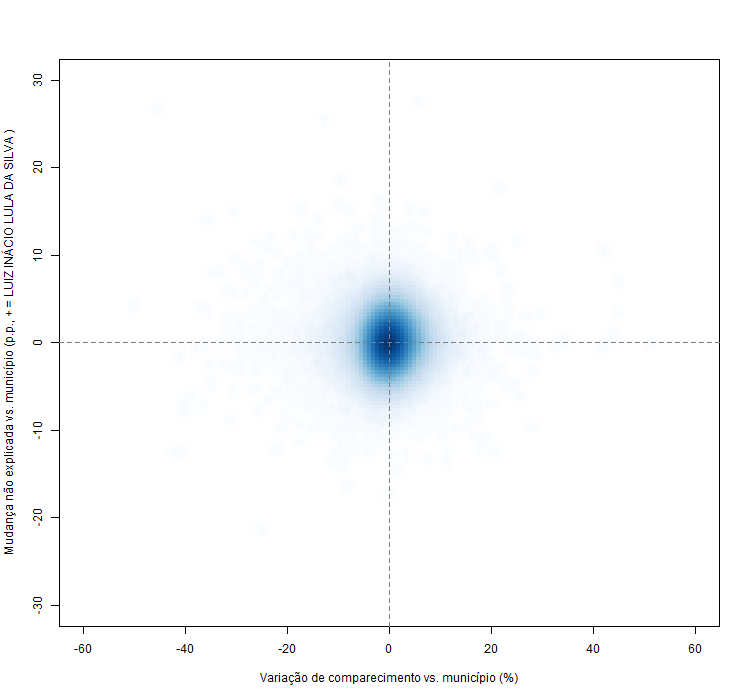
\includegraphics[width=0.85\linewidth]{Figures/T8_dispersao.png}
\caption{Unexplained shift toward Lula (y axis, p.p.) versus turnout change
relative to the municipality (x axis, \%); density plot.}
\label{fig:t8scatter}
\end{figure}

In the validation, T8 found 4 of the 5 inflated sections, and even with the
inserted frauds the overall correlation stayed at $-0.005$: a few inflated
sections do not move the correlation. The list of sections and the symmetry
test are therefore the decisive outputs, and both point to no
one-sided pattern.

%======================================================================
\section{Proposed Further Tests}
\label{sec:proposals}

The strongest tests stop looking only at votes and use the voting
machine's own files and the profile of the electorate
(Table~\ref{tab:proposals}). The first three answer directly whether the
published result is what the machine recorded; the others refine the search
for unusual patterns.

\begin{table*}[ht]
\caption{Proposed tests}
\label{tab:proposals}
\centering\small
\begin{tabular}{@{}c L{3.0cm} L{4.2cm} L{3.4cm} L{5.0cm}@{}}
\toprule
\textbf{\#} & \textbf{Test} & \textbf{What it checks} & \textbf{TSE data} & \textbf{Method} \\
\midrule
1 & BU $\times$ RDV recount & Tally sheet matches the votes recorded one by one & Machine files: BU and RDV & Decode with the published ASN.1 specification \cite{tse2022doc} and recount all sections; 0 divergences expected \\
2 & Digital signature & Published files were not altered after the machine & Machine files: signatures and hashes & Verify the signature of every BU and RDV \\
3 & Printed BU $\times$ published BU & Paper posted at the section equals the tallied file & BU QR code collected by observers & Stratified random sample by state, with CI for the divergence rate \\
4 & Voting rhythm in the log & Votes recorded at a human pace, 8~a.m.--5~p.m. & Machine log & Time between votes, votes per hour, bursts, votes after closing; robust $z$ \\
5 & Releases without biometrics & Excess of voters enabled by code, without fingerprint & Machine log & Rate per section versus municipality, crossed with T8 \\
6 & Machine model & Vote does not depend on equipment model & Log/BU (UE2009 to UE2022) & Regression with municipality fixed effect; model effect should be zero \\
7 & Electorate profile & Section vote consistent with age, sex and schooling & Electorate profile by section & Hierarchical beta-binomial model; posterior predictive checks \\
8 & Panel 2022 $\to$ 2026 & Abrupt changes in the same section between elections & 2022 vote by section & Residual of 2022$\to$2026 change, centred on municipality \\
9 & Percentage spikes (RKD) & Excess of round percentages independent of section size & Vote by section & Resampled kernel density \cite{rozenas2017} \\
10 & Spatial autocorrelation & Clusters of anomalous nearby sections & Polling-place coordinates & Local Moran (LISA) on T6 and T8 residuals \\
11 & Machine-learning detection & Sections similar to simulated fraud scenarios & All of the above & Random forest on synthetic data \cite{zhang2019,cantu2011} \\
12 & Local multimodality & Mixture of two vote regimes within a municipality & Vote by section & Hartigan dip test \cite{hartigan1985} per municipality, BH correction \\
\bottomrule
\end{tabular}
\end{table*}

Tests 1 and 2 have an advantage that no statistical test has: if the RDV
recount matches the BU in every section and all signatures are valid, it is
demonstrated that the published result is the one recorded by the machines,
without depending on any model or assumption about voters.

%======================================================================
\section{Discussion}
\label{sec:discussion}

Regarding \textbf{RQ1}, the 2026 section-level counts follow the expected
regularities: digits, integer percentages, local homogeneity and the
fingerprint behave as in clean data, and the runoff is predicted by the
first round with $R^2=0.93$. Regarding \textbf{RQ2}, deviations are rare
(about 0.01\% of sections for vote tests and 0.15\% for turnout change), most
repeat in both rounds, and their polling-place names point to indigenous
villages, prisons, care homes, sections abroad and a few urban sites, where
the electorate is either homogeneous or changes between rounds. Regarding
\textbf{RQ3}, turnout change and profile change are linked by a small,
monotonic gradient whose sign varies across states, and extreme cases
that gained voters are symmetric between the finalists.

These results agree with the earlier Brazilian studies for 2018
\cite{figueiredo2022} and 2022 \cite{csh2022}. They differ from the Turkish
case \cite{klimek2023}, where extreme cross-round swings in remote areas
favoured the incumbent: in Brazil 2026 the remote sections with extreme
changes do not favour one finalist systematically.

\paragraph{Threats to validity}
\emph{Construct validity}: the tests detect specific forms of manipulation
--- invented numbers, rounding and inflated sections. A small, spread-out
alteration that preserves all these regularities would not be seen; tests 1
to 3 of Section~\ref{sec:proposals} address this. \emph{Internal validity}:
binomial references assume similar voters within a polling place, which
underestimates unanimity in isolated communities (T1); the ecological
regression of T8 does not fit in 9 units; and the classification of
polling places by keywords is approximate. \emph{External validity}: the
results refer to the data published by the TSE on 26~October 2026; later
updates may change marginal counts. \emph{Reliability}: all steps are
scripted and the outputs are saved as files, so the analysis can be
reproduced by third parties.

%======================================================================
\section{Conclusion and Future Work}
\label{sec:conc}

The section-level data of the 2026 Brazilian presidential election do not
show the typical patterns of count manipulation. Digit and
integer-percentage tests are within the expected range for both finalists;
sections of the same polling place are homogeneous; the runoff of each
section is predicted by its first round; the fingerprint has no smear
toward full turnout and full support; and the sections that gained voters
between rounds do not favour one finalist. The deviations found are rare,
mostly repeated in both rounds, and located in sections whose electorate is
homogeneous or changes between rounds.

We recommend: (i) checking the 14 sections flagged by T6 against the tally
sheets in the TSE ``Machine Files'' portal, and verifying whether the four
S\~ao Paulo sections are transit-voting sections; (ii) confirming the type of
the flagged polling places with the official register rather than keywords;
(iii) prioritizing the full BU $\times$ RDV recount and signature
verification, the only tests that confirm the result directly; (iv)
publishing code, data version and results openly; and (v) communicating the
findings as statistical: a flagged section is a point to check, not
evidence of fraud.

%--------------------------------------------------------------------------------
\section*{Acknowledgements}
\addcontentsline{toc}{section}{Acknowledgements}
The author thanks the Graduate Program in Applied Computing of the
University of Bras\'ilia.

\section*{Author contributions}
The author designed the study, wrote the analysis scripts, ran the analyses
and wrote the manuscript.

\phantomsection
\makeatletter
\renewcommand\@biblabel[1]{{\parbox{0.7cm}{[#1]}}}
\makeatother
\renewcommand{\refname}{References}
\bibliography{references}

\balance
\end{document}
